%----------------------------------------------------------------------------------------
%	PACKAGES AND OTHER DOCUMENT CONFIGURATIONS
%----------------------------------------------------------------------------------------

\documentclass[12pt, a4paper, oneside]{Thesis} % Paper size, default font size and one-sided paper

\graphicspath{{./img/}} % Specifies the directory where pictures are stored

\usepackage[square, numbers, comma, sort&compress]{natbib} % Use the natbib reference package - read up on this to edit the reference style; if you want text (e.g. Smith et al., 2012) for the in-text references (instead of numbers), remove 'numbers' 
\hypersetup{urlcolor=black, colorlinks=true} % Colors hyperlinks in blue - change to black if annoying
\title{\ttitle} % Defines the thesis title - don't touch this
\usepackage{caption}
\usepackage{subcaption}
\usepackage{adjustbox}

\renewcommand{\chaptername}{}
\usepackage{titlesec}
\titleformat{\chapter}[hang] 
{\normalfont\huge\bfseries}{\chaptertitlename\thechapter}{1em}{}
\titlespacing{\chapter}{0pt}{0pt}{10pt}% \titlespacing{<command>}{<left>}{<before-sep>}{<after-sep>}[<right>]



%----------------------------------------------------------------------------------------
%      Begin!
%----------------------------------------------------------------------------------------


\begin{document}

\frontmatter % Use roman page numbering style (i, ii, iii, iv...) for the pre-content pages

\setstretch{1.3} % Line spacing of 1.3

% Define the page headers using the FancyHdr package and set up for one-sided printing
\fancyhead{} % Clears all page headers and footers
\rhead{\thepage} % Sets the right side header to show the page number
\lhead{} % Clears the left side page header

\pagestyle{fancy} % Finally, use the "fancy" page style to implement the FancyHdr headers

\newcommand{\HRule}{\rule{\linewidth}{0.5mm}} % New command to make the lines in the title page

%----------------------------------------------------------------------------------------
%	TITLE PAGE
%----------------------------------------------------------------------------------------

\begin{titlepage}
\begin{center}

\textsc{\LARGE \univname}\\[1.5cm] % University name

\HRule \\[0.4cm] % Horizontal line
{\huge \bfseries \ttitle}\\[0.4cm] % Thesis title
\HRule \\[1.5cm] % Horizontal line
 
\begin{minipage}{0.4\textwidth}
\begin{flushleft} \large
\emph{Author:}\\
\href{mailto:j.f.rogers@durham.ac.uk}{\authornames} % Author name - remove the \href bracket to remove the link
\end{flushleft}
\end{minipage}
\begin{minipage}{0.4\textwidth}
\begin{flushright} \large
\emph{Supervisor:} \\
\href{mailto:d.p.halliday@durham.ac.uk}{\supname} % Supervisor name - remove the \href bracket to remove the link  
\end{flushright}
\end{minipage}\\[3cm]

% A thesis submitted in fulfilment of the requirements\\ for the degree of 
\large \textit{\degreename}\\[0.3cm] % University requirement text
\textit{in the}\\[0.4cm]
\groupname\\\deptname\\[2cm] % Research group name and department name
 
{\large \today}\\[1cm] % Date
\includegraphics{Logo} % University/department logo - uncomment to place it
 
\vfill
\end{center}

\end{titlepage}


%----------------------------------------------------------------------------------------
%	ABSTRACT PAGE
%----------------------------------------------------------------------------------------

\addtotoc{Abstract} % Add the "Abstract" page entry to the Contents

\abstract{\addtocontents{toc}{\vspace{1em}} % Add a gap in the Contents, for aesthetics

We look at the four ternary phase Diagrams of CZTS at 298k, reducing them to their simplest form, from this we construct a three dimensional quaternary phase diagram in order to find the thermodynamic `location' of CZTS.
}

\clearpage % Start a new page


%----------------------------------------------------------------------------------------
%	LIST OF CONTENTS/FIGURES/TABLES PAGES
%----------------------------------------------------------------------------------------

\pagestyle{fancy} % The page style headers have been "empty" all this time, now use the "fancy" headers as defined before to bring them back

\lhead{\emph{Contents}} % Set the left side page header to "Contents"
\tableofcontents % Write out the Table of Contents

%----------------------------------------------------------------------------------------
%	THESIS CONTENT - CHAPTERS
%----------------------------------------------------------------------------------------

\mainmatter % Begin numeric (1,2,3...) page numbering

\pagestyle{fancy} % Return the page headers back to the "fancy" style

% Include the chapters of the thesis as separate files from the Chapters folder
% Uncomment the lines as you write the chapters

% Chapter Template

\chapter{Introduction} % Main chapter title

\label{Chapter1} % Change X to a consecutive number; for referencing this chapter elsewhere, use \ref{ChapterX}

\lhead{\emph{Introduction}} % Change X to a consecutive number; this is for the header on each page - perhaps a shortened title

%----------------------------------------------------------------------------------------
%	SECTION 1
%----------------------------------------------------------------------------------------

\section{History \& Background}

The extent of solar energy reaching the earth's surface produces an energy supply potential far exceeding the energy requirement of our planet's needs by three orders of magnitude \citep{Morton2006}. However, this resource has not been harvested to a great value - currently only 0.1\% of worldwide power generation is met by photovoltaic supply \citep{Mitzi2011}.  This is largely due to the previous high cost difference between Solar and more conventional power generation techniques. As such, to gain any real impact upon worldwide power consumption, photovoltaic cells must fit the following characteristics: must be cost effective, highly abundant, provide a supply for a long lifetime before degradation, and have a high power efficiency.


The 1839 discovery of the Photovoltaic effect by Edmund Becquerel \citep{Nelson2003}, whilst experimenting with electrolytic cells, was the first step into the field of solar power and technology, and the first of several discoveries along the path to using the sun as an energy source for power. Following this, in 1883, Charles Fritts \citep{Fritts1883} developed the first solid state solar cell, by coating selenium with a thin layer of gold to form the junctions, this was then followed by a series of successive discoveries between 1839 and 1941 led to the development and patenting of the first "Light Sensitive Device", by Russell Ohl in 1946, a modern junction semiconductor solar cell \citep{Green2009a}. 

This melt grown junction device had less than 1\% efficiency, and was succeeded by a device built by Kingsbury and Ohl produced through Helium-bombardment, boasting an efficiency of ~1\% in 1952 \citep{Green2009a}. Further developments in semiconductor photovoltaics led to efficiencies reaching 14\%, but at costs of up to \$250 per watt (compared to \$2-3 for a coal plant) by 1954. Due to the move to integrated circuits within the semiconductor industry in the late 1970's, the price of silicon cells dropped to \$100 per watt.

Further improvements to  solar cells have both improved efficiency and reduced the cost, with large arrays able to be built at below \$2.24/W$_p$ \citep{EricWesoff}, and as of September 2013, up to 44.7\% efficiency, using a GaInP/GaAs/\\GaInAsP/GaInAs multi-junction \citep{ISI:000331334400001}.

%-----------------------------------
%	SUBSECTION 1
%-----------------------------------

\subsection{Thin Film}

Thin film solar cells were originally developed for usage in small scale applications such as calculators, but are now available for usage in much larger scale installations such as car charging systems; produced by sandwiching a film of photovoltaic material between two panes of glass. 

Thin Film materials are semiconductors which overcome on of the limitations of a standard crystalline Silicon semiconductor, as they have a direct band gap - this results in a high light absorption coefficient meaning that for solar energy to be harvested, thin films have a lower material requirement than that required by standard semiconductor solar cells. When using a thin film crystal, this comes with a reduction of the efficiency of the the bulk material (20\% down from 25\%, in the case of Amorphous Silicon against Silicon Heterostructure cells), and a similar difference in efficiency is demonstrated when comparing thin film compounds to a crystalline silicon cell - CIGS devices have a record efficiency of 23.3\%, whilst Single crystal Silicon Devices have a record efficiency of 27.6\% \citep{Photovoltaics2014}. Due to the reduced need for component elements, there is a lower environmental impact and reduced payback time (currently 75\% of standard multi-crystalline Solar Cells, at 3 years rather than 4; projected to 50\% of future multi-crystalline cells) \citep{Photovoltaics}, however this is countered currently by a much lower efficiency than standard solar cells. In addition to this, a furthher advantage of thin film materials over Silicon is the reduced quality requirements of the materials - thin film materials display a tolerance to grain boundaries and defects \citep{Siebentritt2006}. 

%----------------------------------------------------------------------------------------
%	SECTION 2
%----------------------------------------------------------------------------------------
\section{CZTS}

Strong candidate compounds for Thin Film Solar Cells are Cadmium Telluride (CdTe) and Copper Indium Gallium Selenide (CIGS), showing promise as general purpose cells and seeing high commercial success, in November Hanergy unveiled a manufacturing facility amounting to 5.25GW capacity \citep{Mark}, and further to this, began building another manufacturing facility with 3GW capacity \citep{FinlayColville}; however recent concerns have been voiced over the cost, due to the abundance of the materials used in these compounds. In 2005, the costs of Indium increased to over \$1000/kg from \$200/kg, due to its' usage in displays \citep{Feltrin2008}. Tellurium is similarly high priced due to its scarcity being similar to that of Gold. The combinations of these with the Toxicity of Cadmium lead to the requirement of a new Compound, that would fulfill the requirements of a solar cell.

Copper Zinc Tin Sulphide (CZTS) is seen as the compound of choice for solving the problems laid out above, as it is produced from highly abundant, non-toxic materials - the abundance of Tin and Zinc in the earth's crust is 1500 times and 45 times greater than that of Indium; leading to a much lower cost, two orders of magnitude smaller than that of Indium \citep{Wadia2009,Wang2011}.
The first solar cell using CZTS were produced in 1997, with an efficiency of 2.3\%, and in November 2013 Solar frontier, a Japanese thin-film company developed a CZTS solar cell with 12.6\% efficiency \citep{Wang2013}.

%-----------------------------------
%	SUBSECTION 1
%-----------------------------------

\subsection{Complexity}

CZTS as a mineral has been known to geologists since 1958 \citep{Kissin1989}, however it was only discovered to have the photovoltaic effect in 1988 \citep{Ito1988}. Its' structure is similar to that of the chalcopyrite material CuInS$_2$, however in place of the group 13 valence 3 Indium, is half group 14 valence 4 Tin, and half group 12 valence 2 Zinc, maintaining an average valence of 3. CZTS is a complex material to examine, as it exists as one of two very similar principal structures - Stannite and Kesterite, whose structures are very similar, with a rearrangement of the positions of Cu and Zn \citep{Schorr2007}. CZTS is mainly found to occur in the Kesterite phase, due to its thermodynamic stability (indeed, pure Kesterite is the most stable tin containing sulphide \citep{moh1975}) in comparison to the Stannite phase, and can be produced from solid state reactions between Zinc Sulphide, Copper (II) Sulphide, and Tin Sulphide.

%----------------------------------------------------------------------------------------
%	SECTION 3
%----------------------------------------------------------------------------------------
\section{Methods Of Production}

The methods used to produce thin film materials may be categorised as either a single stage or two stage reaction. The single stage reaction produces the desired material in a single step, such as an all-in heating method, where all the required materials are evaporated onto a substrate. This method has produced good results for CIGS devices, though has not proven as beneficial to CZTS devices \citep{scragg2011copper}. Two stage processes encompass the majority of preparation methods, and consists of first preparing a precursor material, generally at room temperature and containing only the metallic elements used in the compound, or all of the elements in the compound in an uncrystallized form. Subsequently, the precursor is heated in an atmosphere of Sulphur (Sulphurisation), inducing formation or crystallisation of the required phase.

%-----------------------------------
%	SUBSECTION 1
%-----------------------------------
\subsection{Vacuum Methods}

%-----------------------------------
%	SUBSUBSECTION 1
%-----------------------------------  
\subsubsection{Sputtering}
Sputtering is a method of physical vapor deposition, through ejection of a material from a `target' onto a `substrate' such as a silicon wafer. This ejection occurs by running a charge to an anode and cathode (with the cathode formed of the material to be sputtered), and pushing a gas through the sputtering chamber at a high pressure. The sputtered ions may travel ballistically from the target to the substrate, or at higher pressures the gas may act as a moderator and allow the sputtered material to diffuse through the system, condensing and adhering to the substrate after undergoing a random walk.
Often an electromagnet is used to keep plasma particles close to the surface of the sputter target - Rf sputtering is the process of using an RF power source in order to ionize the the gaseous atoms. Once the ions contact the target material, it is broken into small pieces which travel to the substrate, forming a coating.
\begin{figure}
\centering
\includegraphics[width=80mm]{sputtering.png}
\caption{A general method for sputtering, \citep{wikipedia2014}}
    \label{fig:Sputtering}
\end{figure}
An advantage of this method is that metals with high melting points are easily sputtered, whilst evaporation of these materials is problematic. This method causes the film to have a composition very close to that of the source material, with a slight difference due to the spreading of various elements because of their mass differences. These films have a higher adhesion rate than evaporated films, and due to the low temperature they work at, have no hot parts.

This method has achieved a 6.77\% efficiency over a 0.15cm$^2$ active area, representing one of the highest efficiency values for a pure CTZ film \citep{Mitzi2011}. 
%-----------------------------------
%	SUBSUBSECTION 2
%-----------------------------------
\subsubsection{Co-Evaporation}

The principle deposition method used in many of the early kesterite cells, which was chosen after it's previous successes with CIGSSe materials.
The first functional evaporated kesterite device (power efficiency of 0.66\%, found in 1997) , and subsequent multilayer structures were evaporated at a temperature of 150$^\circ$C, then subject to sulphurization at 500$^\circ$C in 5\% nitrogen in a hydrazine atmosphere.

Later deposition methods substituted ZnS as opposed to Zn, for the bottom layer and an increase in initial temperature to 400$^\circ$C - this lead to 2.62\% efficiency \citep{Todorov2010}.

%-----------------------------------
%	SUBSECTION 2
%-----------------------------------
\subsection{Non-Vacuum Methods}
%-----------------------------------
%	SUBSUBSECTION 1
%-----------------------------------
\subsubsection{Electrodeposition}
The process of using electrical current to reduce a solution of dissolved metal ions to form a metal coating onto an electrode. This is used to build up several layers of elements onto a substrate to form the thin film solar cell. This process has the side effect of changing the the chemical physical and mechanical properties of the item to be plated, which may have detrimental or unwanted side effects. This is an attractive method for large-scale applications, due to the large number of cells which may be produced simultaneously. Early work in the field began by successively plating each of the metals onto a substrate, before sulfurization with elemental Sulphur. This led to an efficiency of ~0.8\% \citep{Scragg2008}, however limitations on device performance included the high series resistance, high shunt conductance and substantial recombination in the space charge region. Other efforts resulted in poor layer adhesion to the substrate, solved through addition of Palladium to the substrate leading to 0.98\% efficiency. The current record efficiency for an electrodeposited CZTS device is 3.4\%, using a Solid state reaction of Cu$_2$SnS$_3$ and ZnS, at 550K.



%----------------------------------------------------------------------------------------
%	SECTION 4
%----------------------------------------------------------------------------------------

\section{Theory}



%-----------------------------------
%	SUBSECTION 1
%-----------------------------------

\subsection{Photovoltaic Effect}

All solar cells work on the principle of the photovoltaic effect, the one step-conversion process which generates electrical energy from light. Photons in sunlight are incident upon the solar panel and are absorbed. The energy of these photons is sufficient to excite electrons within the semiconductor into higher levels where they are free to move, forming electron-hole pairs. In other materials, the electrons may quickly  relax back to ground state, however in the photovoltaic device there exists an asymmetry which pulls apart the electron-hole pair before relaxation can occur, this occurs at the p-n junction and produces a potential difference, and as such a voltage.


%-----------------------------------
%	SUBSECTION 2
%-----------------------------------

\subsection{P-N Junctions}

A p-n junction can be formed from a single crystal or material which is doped into two regions: one doped with acceptor impurities to produce a p-region, with holes as the charge carrier; the other doped with donor impurities to produce an n-region, with electrons as the charge carrier; the interface between these two regions can be less than 10$^-4$ cm thick \citep{Kittel2004}.  In the case of CZTS, rather than doping a single material, a combination of materials is used: many devices use a thin film of CZTS on a Molybdenum coated soda lime glass. Upon the CZTS is a CdS n-type layer (forming the p-n junction), and subsequently an i-ZnO/AL:ZnO layer acting as a window layer;The electrical contacts ion this set up are the Soda Lime Glass, and ZnO layers \citep{Wang2011}.
If an external voltage is applied such that the n-type region of the material is the negative terminal, we observe the electrons and holes move towards one another at the junction and recombine -this is  known as the forward bias, and is the basis for a light emitting diode.
If the polarity of the applied voltage is reversed, then electrons and holes moving away from the junction is observed and the material behaves as an insulator with virtually no current flow -  this is the reverse bias and basis for a photodetector \citep{Askeland2010}. Under illumination we find that the charge separation will continue to occur, despite there being no applied voltage. These moving charges can be detected as an external photocurrent, or we can measure this as a potential difference, and as such given a material with the correct band gap energy (1.6eV to 3.1eV, CZTS has a band gap of ~1.5eV \citep{JJAP.48.090202,Katagiri2001}) solar cells can be produced.

\input{Sections/Method} 
% Chapter Template

\chapter{Results} % Main chapter title

\label{Chapter3} % Change 3 to a consecutive number; for referencing this chapter elsewhere, use \ref{Chapter3}

\lhead{\emph{Results}} % Change X to a consecutive number; this is for the header on each page - perhaps a shortened title

%----------------------------------------------------------------------------------------
%   SECTION 1
%----------------------------------------------------------------------------------------

\section{Ternary Diagrams}

\begin{figure}
\centering
\begin{subfigure}{80mm}
  \centering
    \includegraphics[width=80mm]{triangleplot_CUZNS298.png}
    \caption{Cu, Zn, S Ternary Diagram}
    \label{fig:CuZnS}
\end{subfigure}%
\begin{subfigure}{80mm}
 \centering
    \includegraphics[width=80mm]{triangleplot_CUZNSN298.png}
    \caption{Cu, Zn, Sn Ternary Diagram}
    \label{fig:CuZnSn}
\end{subfigure}
\begin{subfigure}{80mm}
 \centering
    \includegraphics[width=80mm]{triangleplot_CUSNS298.png}
    \caption{Cu, Sn, S Ternary Diagram}
    \label{fig:CuSnS}
\end{subfigure}
\caption{Ternary Diagrams of the remaining face, post 'Tie-line' calculations.}
\label{fig:RemainingFaces}
\end{figure}

In Figures 1 and 3, we see completed Ternary Phase Diagrams for the four faces of the original quaternary diagram - with all crossing points removed and the stable pahses of the diagrams present.
These allow us to further produce a Quaternary diagram with indicative 'tie-phases', and as such locate the thermodynamic area we are most likely to find CZTS in. An example of one of the possible candidate 'tie-phases' is presented in figure 2. This and four other candidate 'tie-phases' were examined to find a 'tie-phase' with the correct 2:1 ratio of sulphur to the other elements present within CZTS. Through determination of the ratios, I found only one acceptable candidate: $ZnS$, $Sns_2$, $Cu_2S$, though another would fit the general ratio, that of $ZnS$, $Sn_2s_3$, $Cu_2S$ however, this did not have the correct ratio of Copper, Zinc and Tin and as such was dismissed.

Presented in figure 4 is a diagram demonstrating the theoretical area where CZTS is most likely to occur; also presented are the areas which are generally either more "rich" or "poor" in on of the elements. This fits with the work presented by Olekseyuk in 2004.\citep{Olekseyuk2004}

%----------------------------------------------------------------------------------------
%   SECTION 2
%----------------------------------------------------------------------------------------

\section{Quaternary Diagram}

\begin{figure}
\centering
 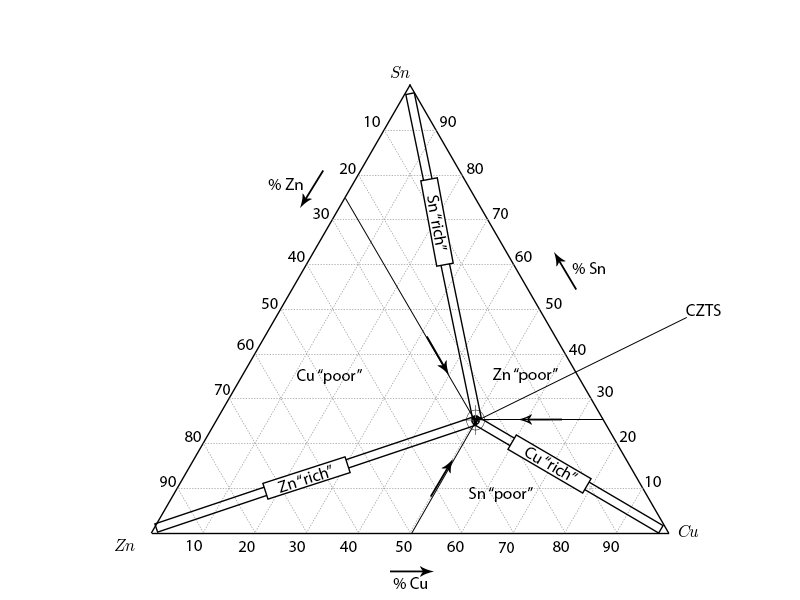
\includegraphics[width=80mm]{ZnSSn2S3Cu2S-general}
    \caption{Location of CZTS, and labelled secondary phases.}
    \label{fig:ZnSSn2S3Cu2S}
\end{figure}

%\input{Sections/Chapter4} 
%\input{Sections/Chapter5} 
%\input{Sections/Chapter6} 
%\input{Sections/Chapter7} 

%----------------------------------------------------------------------------------------
%	ACKNOWLEDGEMENTS
%----------------------------------------------------------------------------------------

\setstretch{1.3} % Reset the line-spacing to 1.3 for body text (if it has changed)

\acknowledgements{\addtocontents{toc}{\vspace{1em}} % Add a gap in the Contents, for aesthetics

The acknowledgements and the people to thank go here, don't forget to include your project advisor\ldots
}
\clearpage % Start a new page

%----------------------------------------------------------------------------------------
%	BIBLIOGRAPHY
%----------------------------------------------------------------------------------------

\label{References}

\lhead{\emph{References}} % Change the page header to say "Bibliography"

\bibliographystyle{apsrev} % Use the "unsrtnat" BibTeX style for formatting the Bibliography

\bibliography{../library} % The references (bibliography) information are stored in the file named "Bibliography.bib"

  

%----------------------------------------------------------------------------------------
%	THESIS CONTENT - APPENDICES
%----------------------------------------------------------------------------------------

\addtocontents{toc}{\vspace{2em}} % Add a gap in the Contents, for aesthetics

\appendix % Cue to tell LaTeX that the following 'chapters' are Appendices

% Include the appendices of the thesis as separate files from the Appendices folder
% Uncomment the lines as you write the Appendices

% Appendix A

\chapter{Appendix Title Here} % Main appendix title

\label{AppendixA} % For referencing this appendix elsewhere, use \ref{AppendixA}

\lhead{Appendix A. \emph{Appendix Title Here}} % This is for the header on each page - perhaps a shortened title

\begin{figure}[t]
\centering
\begin{subfigure}{70mm}
  \centering
    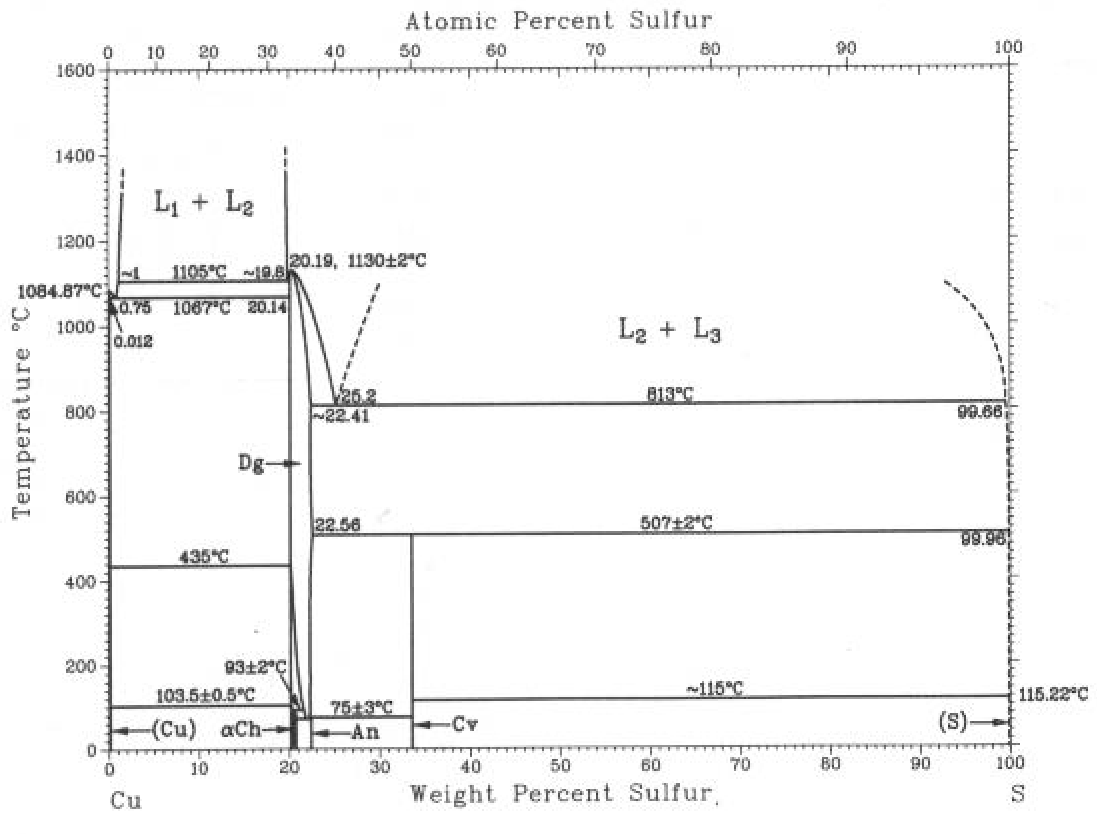
\includegraphics[width=70mm]{CuSAlloyDiag.png}
    \caption{Cu, S Binary Phase Diagram\citep{Hay2000}}
    \label{fig:CuS}
\end{subfigure}%
\begin{subfigure}{70mm}
 \centering
    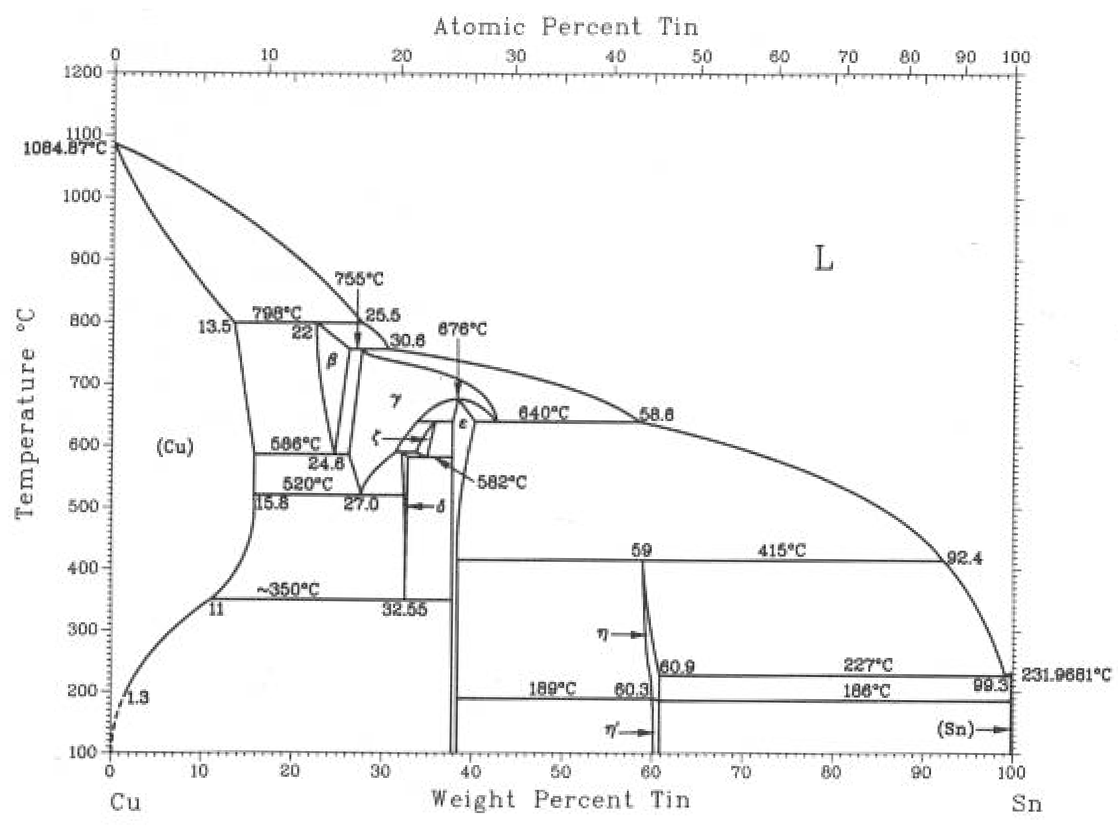
\includegraphics[width=70mm]{CuSnAlloyDiag.png}
    \caption{Cu, Sn Binary Phase Diagram\citep{Hay2000}}
    \label{fig:CuSn}
\end{subfigure}
\begin{subfigure}{70mm}
 \centering
    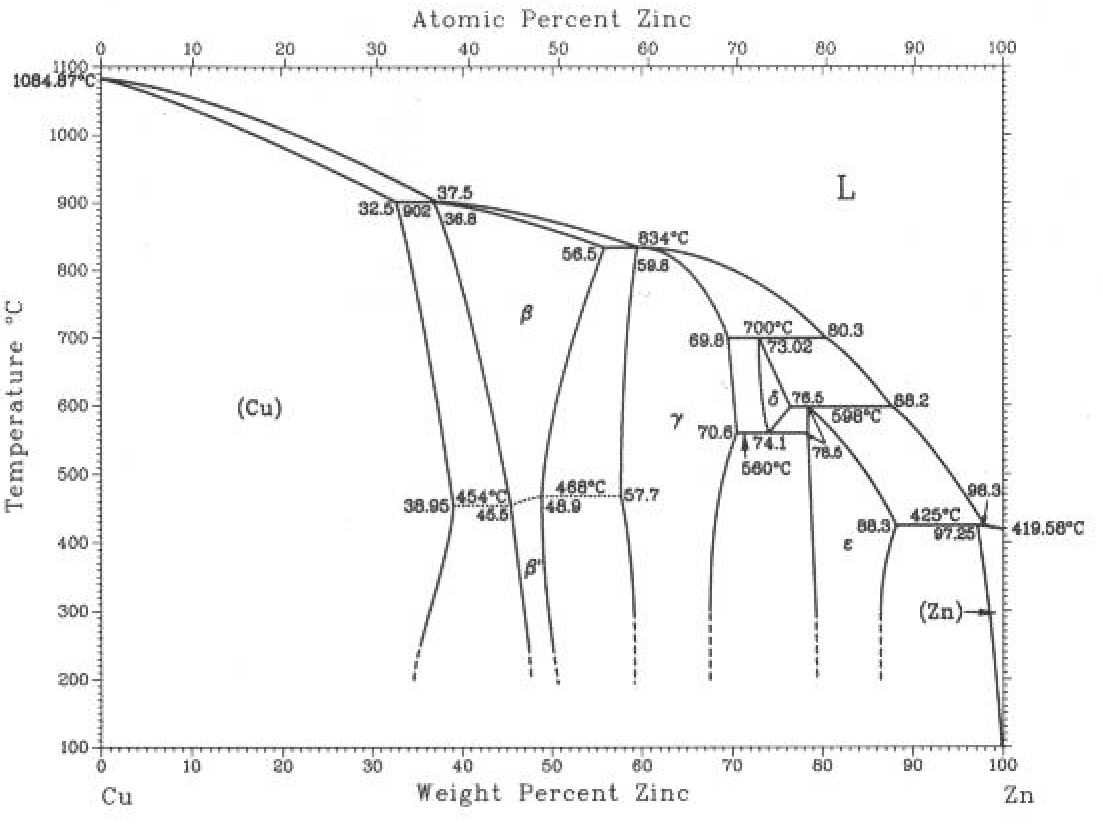
\includegraphics[width=70mm]{CuZnAlloyDiag.png}
    \caption{Cu, Zn Binary Phase Diagram\citep{Hay2000}}
    \label{fig:CuZn}
\end{subfigure}
\begin{subfigure}{70mm}
 \centering
    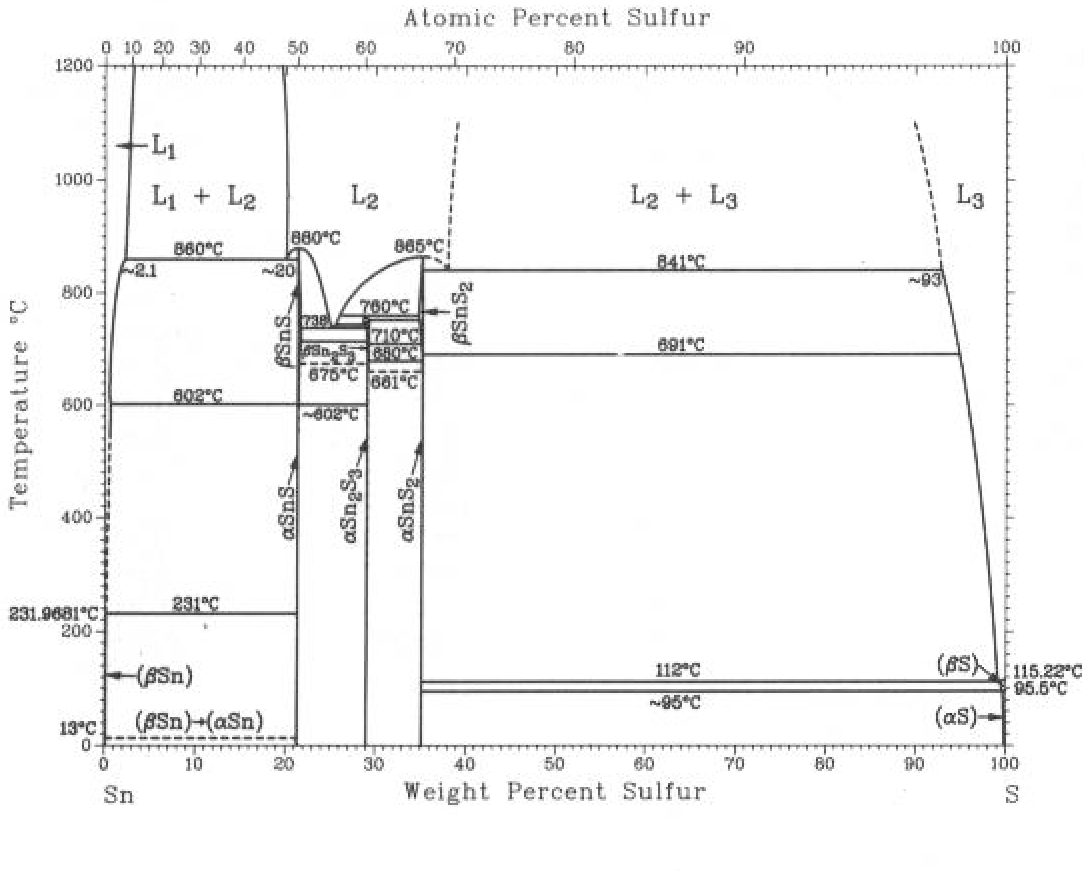
\includegraphics[width=70mm]{SnSAlloyDiag.png}
    \caption{Sn, S Binary Phase Diagram\citep{Hay2000}}
    \label{fig:SnS}
\end{subfigure}
\begin{subfigure}{70mm}
 \centering
    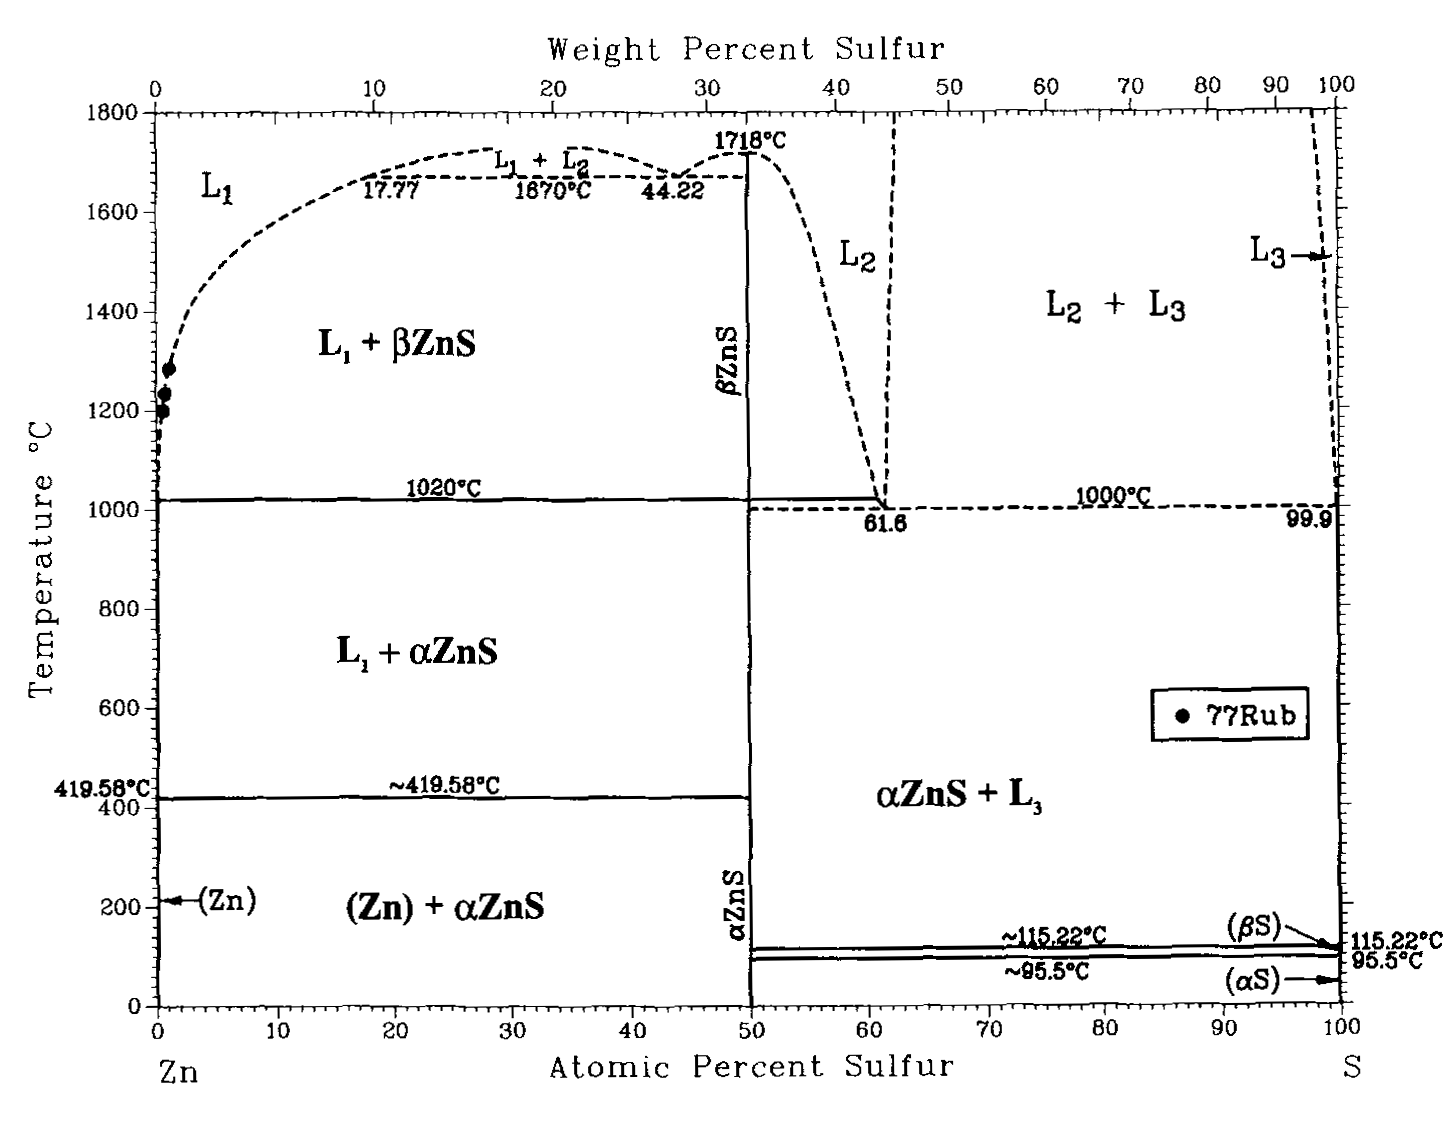
\includegraphics[width=70mm]{ZnSAlloyDiag.png}
    \caption{Zn, S Binary Phase Diagram\citep{Sharma1996}}
    \label{fig:ZnS}
\end{subfigure}
\begin{subfigure}{70mm}
 \centering
    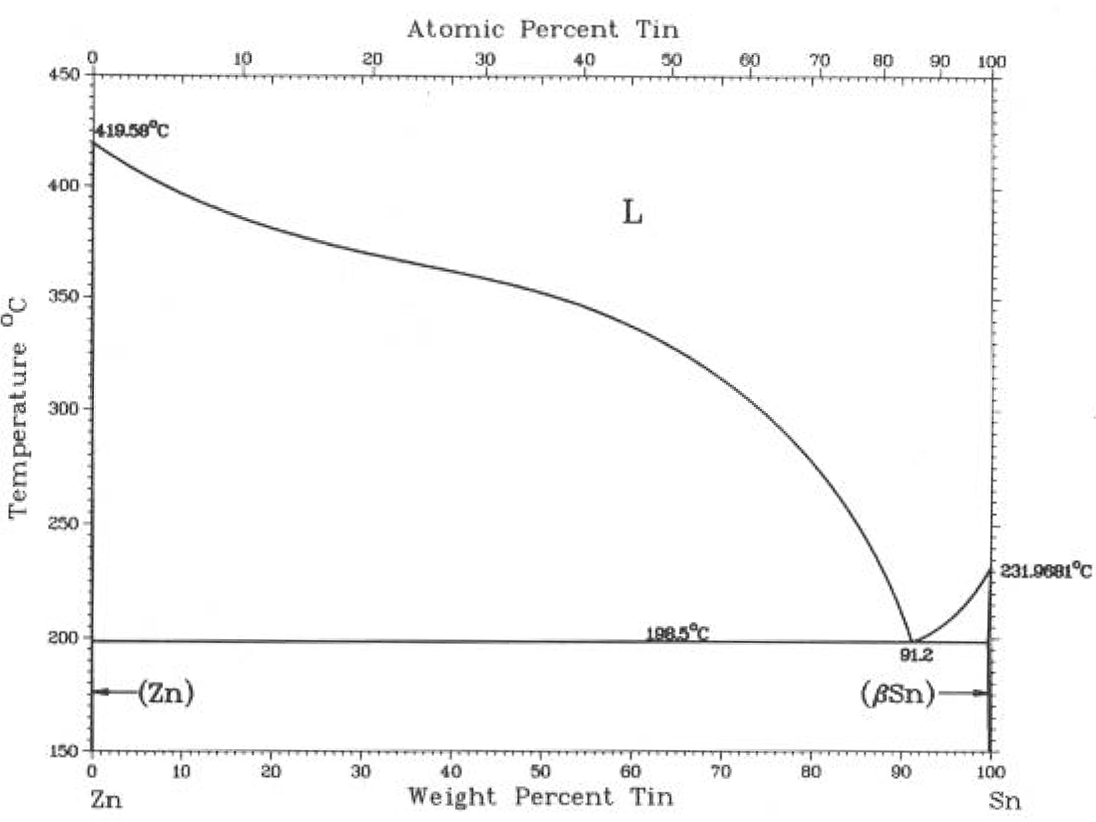
\includegraphics[width=70mm]{ZnSnAlloyDiag.png}
    \caption{Zn, Sn Binary Phase Diagram\citep{Hay2000}}
    \label{fig:ZnSn}
\end{subfigure}
\caption{Binary Alloy Phase Diagrams Used in the calculation of the Ternary Phase Diagrams.}
\label{fig:BinaryAlloyPhaseDiagrams}
\end{figure}
%% Appendix A

\chapter{Binary Phase Diagrams} % Main appendix title

\label{AppendixB} % For referencing this appendix elsewhere, use \ref{AppendixA}

\lhead{Appendix B. \emph{Binary Phase Diagrams}} % This is for the header on each page - perhaps a shortened title

\begin{figure}[h]
\centering
\begin{subfigure}{70mm}
  \centering
    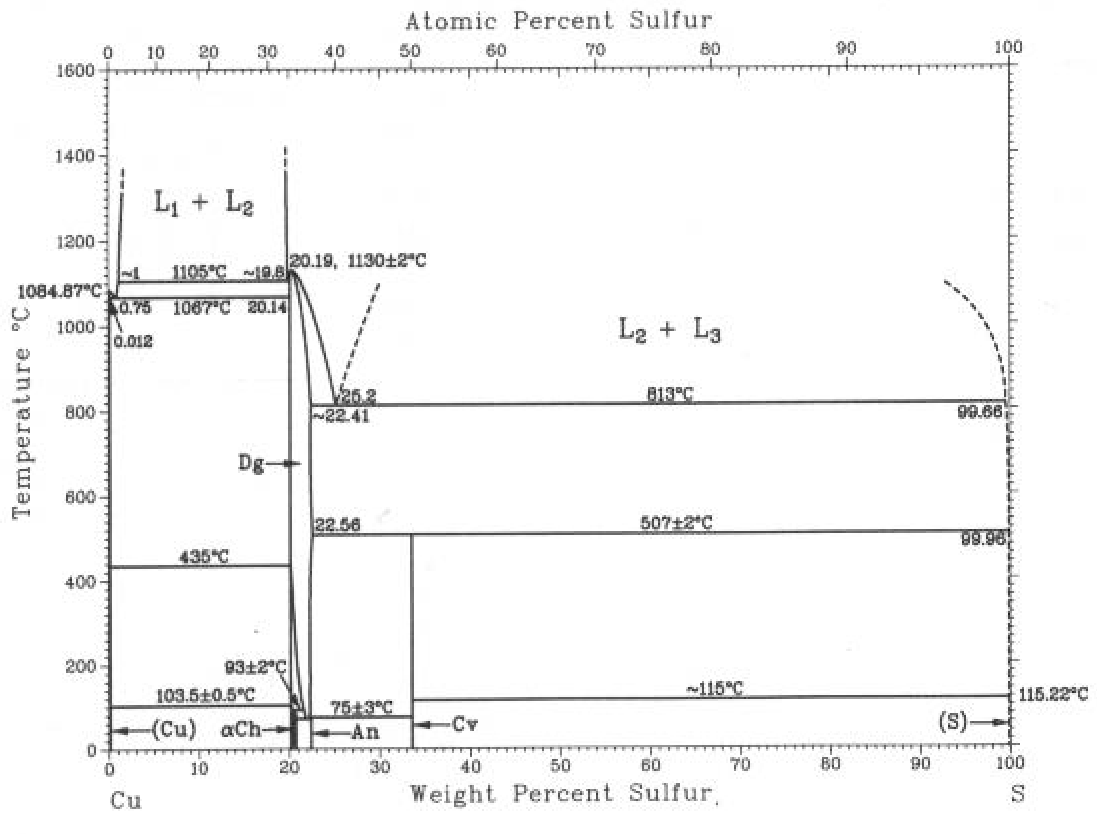
\includegraphics[width=70mm]{CuSAlloyDiag.png}
    \caption{Cu, S Binary Phase Diagram\citep{Hay2000}}
    \label{fig:CuS}
\end{subfigure}%
\begin{subfigure}{70mm}
 \centering
    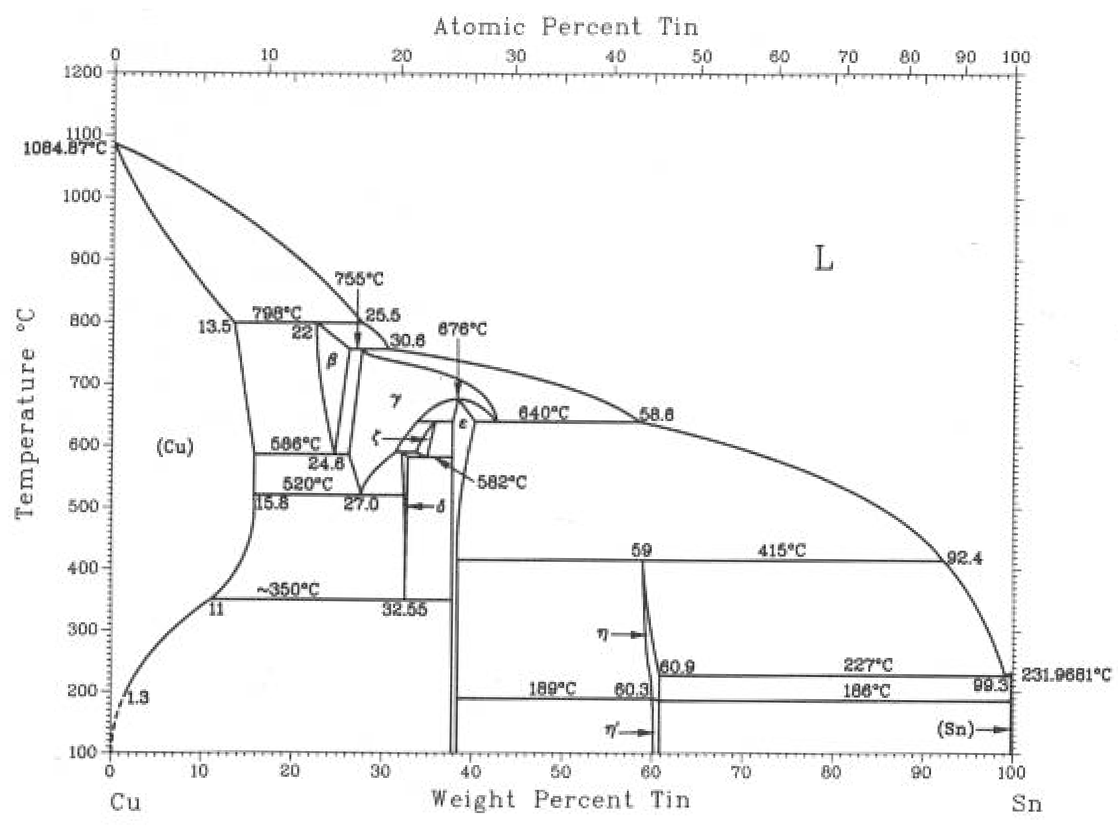
\includegraphics[width=70mm]{CuSnAlloyDiag.png}
    \caption{Cu, Sn Binary Phase Diagram\citep{Hay2000}}
    \label{fig:CuSn}
\end{subfigure}
\begin{subfigure}{70mm}
 \centering
    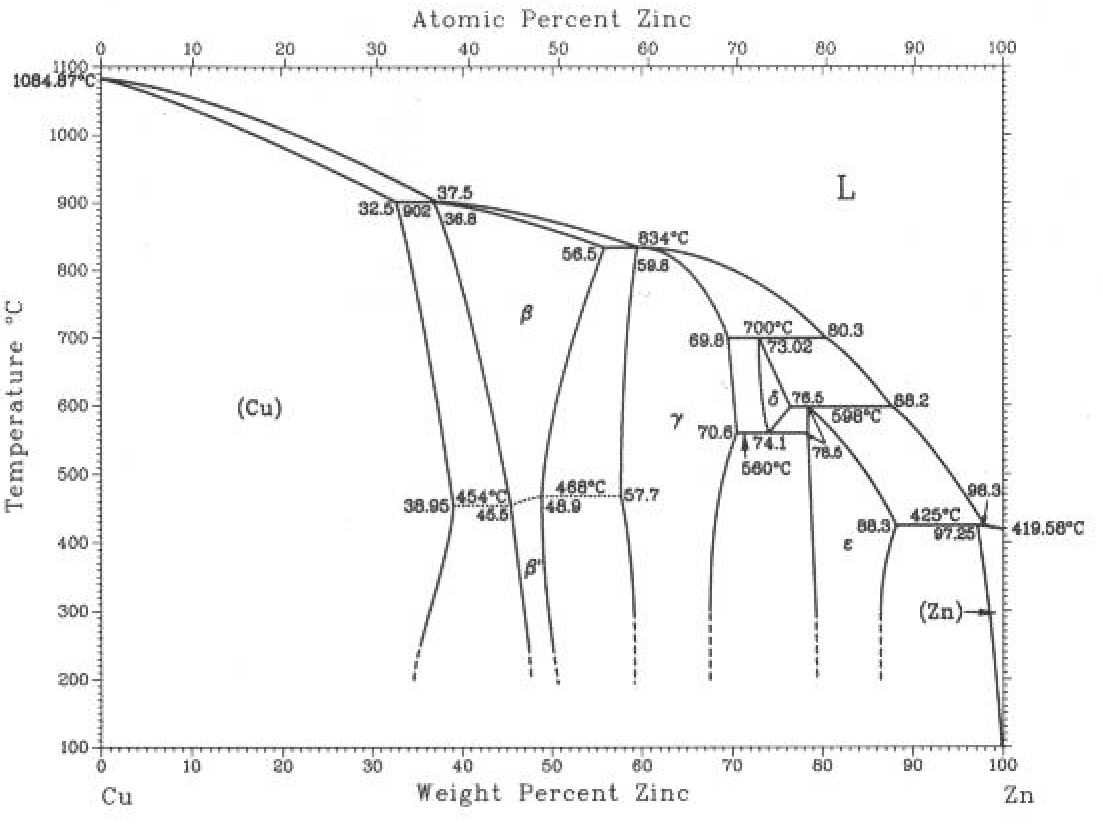
\includegraphics[width=70mm]{CuZnAlloyDiag.png}
    \caption{Cu, Zn Binary Phase Diagram\citep{Hay2000}}
    \label{fig:CuZn}
\end{subfigure}
\begin{subfigure}{70mm}
 \centering
    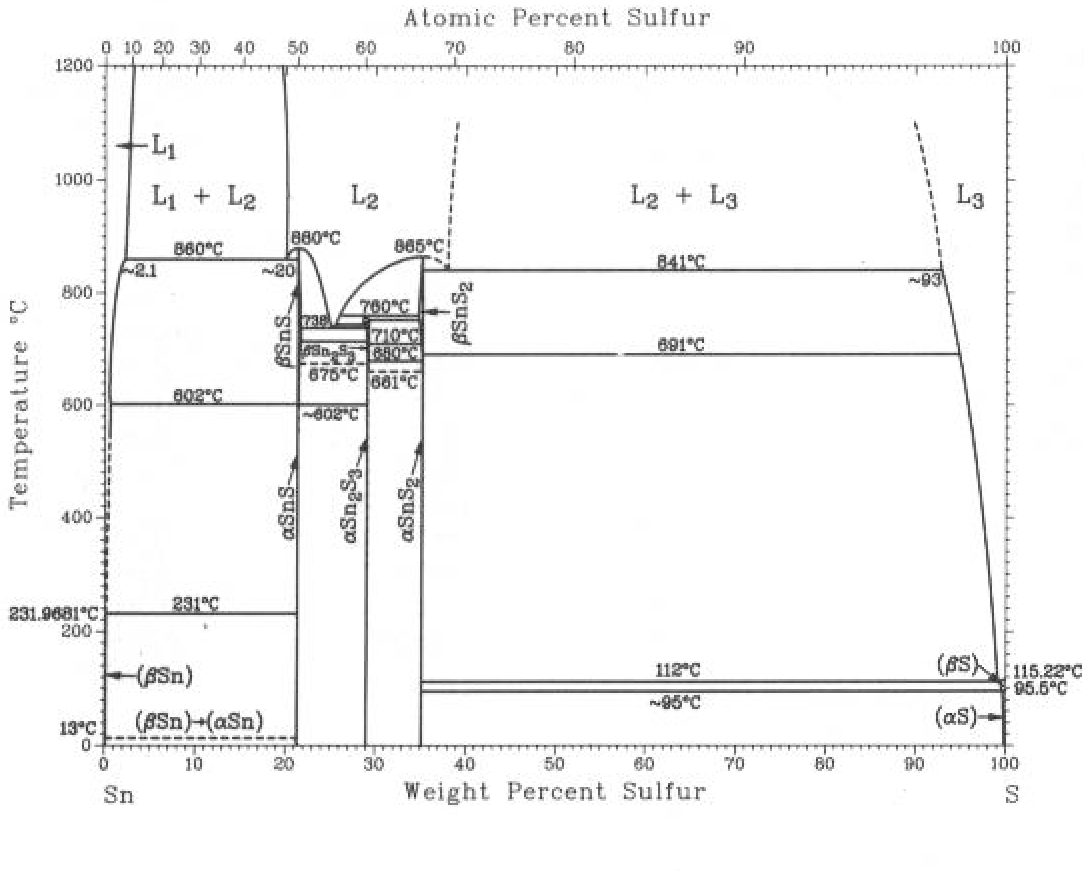
\includegraphics[width=70mm]{SnSAlloyDiag.png}
    \caption{Sn, S Binary Phase Diagram\citep{Hay2000}}
    \label{fig:SnS}
\end{subfigure}
\begin{subfigure}{70mm}
 \centering
    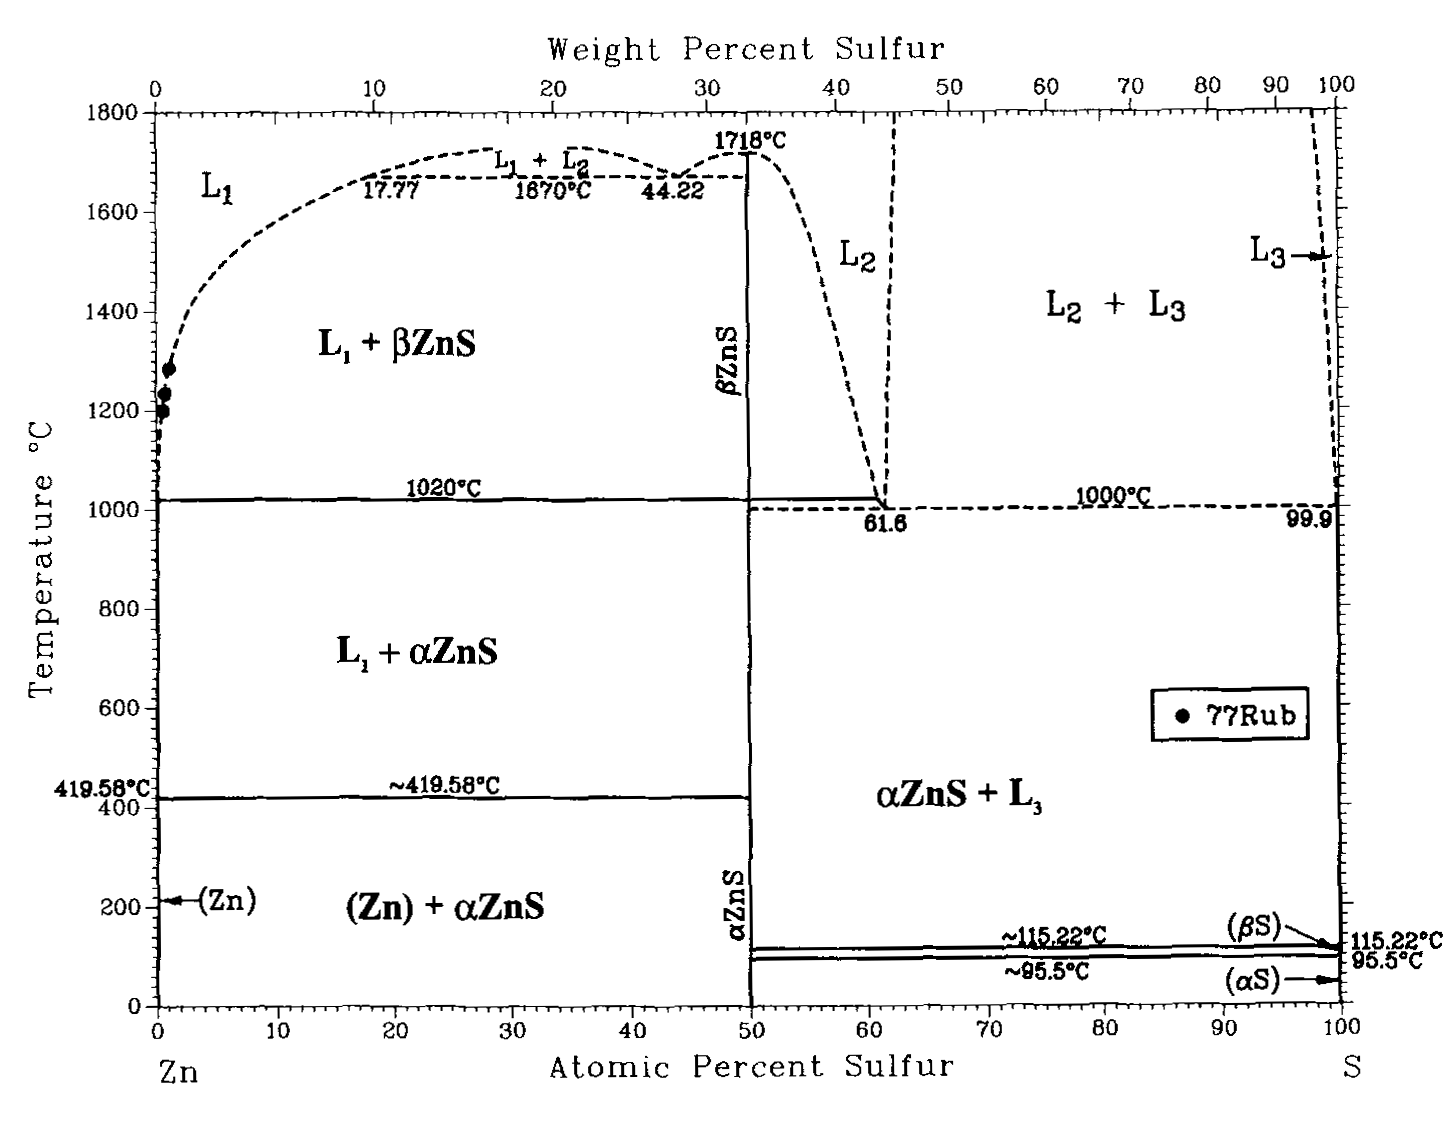
\includegraphics[width=70mm]{ZnSAlloyDiag.png}
    \caption{Zn, S Binary Phase Diagram\citep{Sharma1996}}
    \label{fig:ZnS}
\end{subfigure}
\begin{subfigure}{70mm}
 \centering
    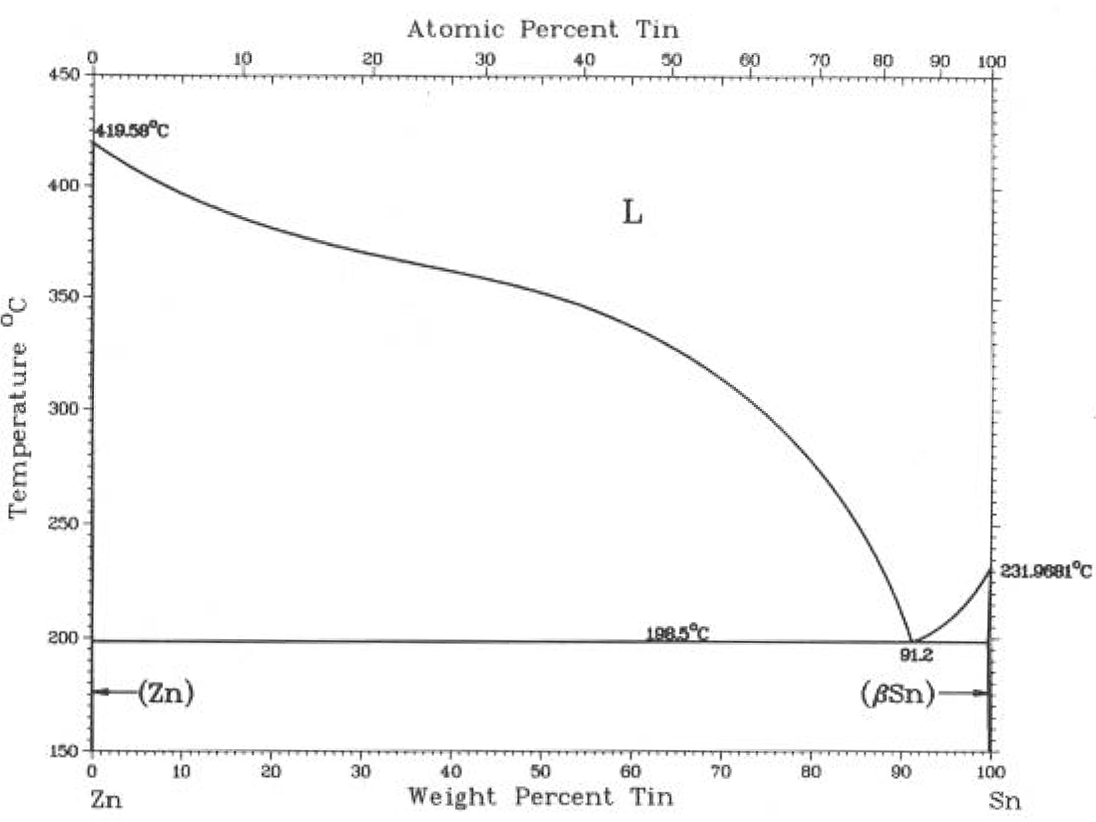
\includegraphics[width=70mm]{ZnSnAlloyDiag.png}
    \caption{Zn, Sn Binary Phase Diagram\citep{Hay2000}}
    \label{fig:ZnSn}
\end{subfigure}
\caption{Binary Alloy Phase Diagrams Used in the calculation of the Ternary Phase Diagrams.}
\label{fig:BinaryAlloyPhaseDiagrams}
\end{figure}
%% Appendix A

\chapter{Quaternary Phase Diagram} % Main appendix title

\label{AppendixC} % For referencing this appendix elsewhere, use \ref{AppendixA}

\lhead{Appendix C. \emph{Quaternary Phase Diagram}} % This is for the header on each page - perhaps a shortened title

\begin{figure}
	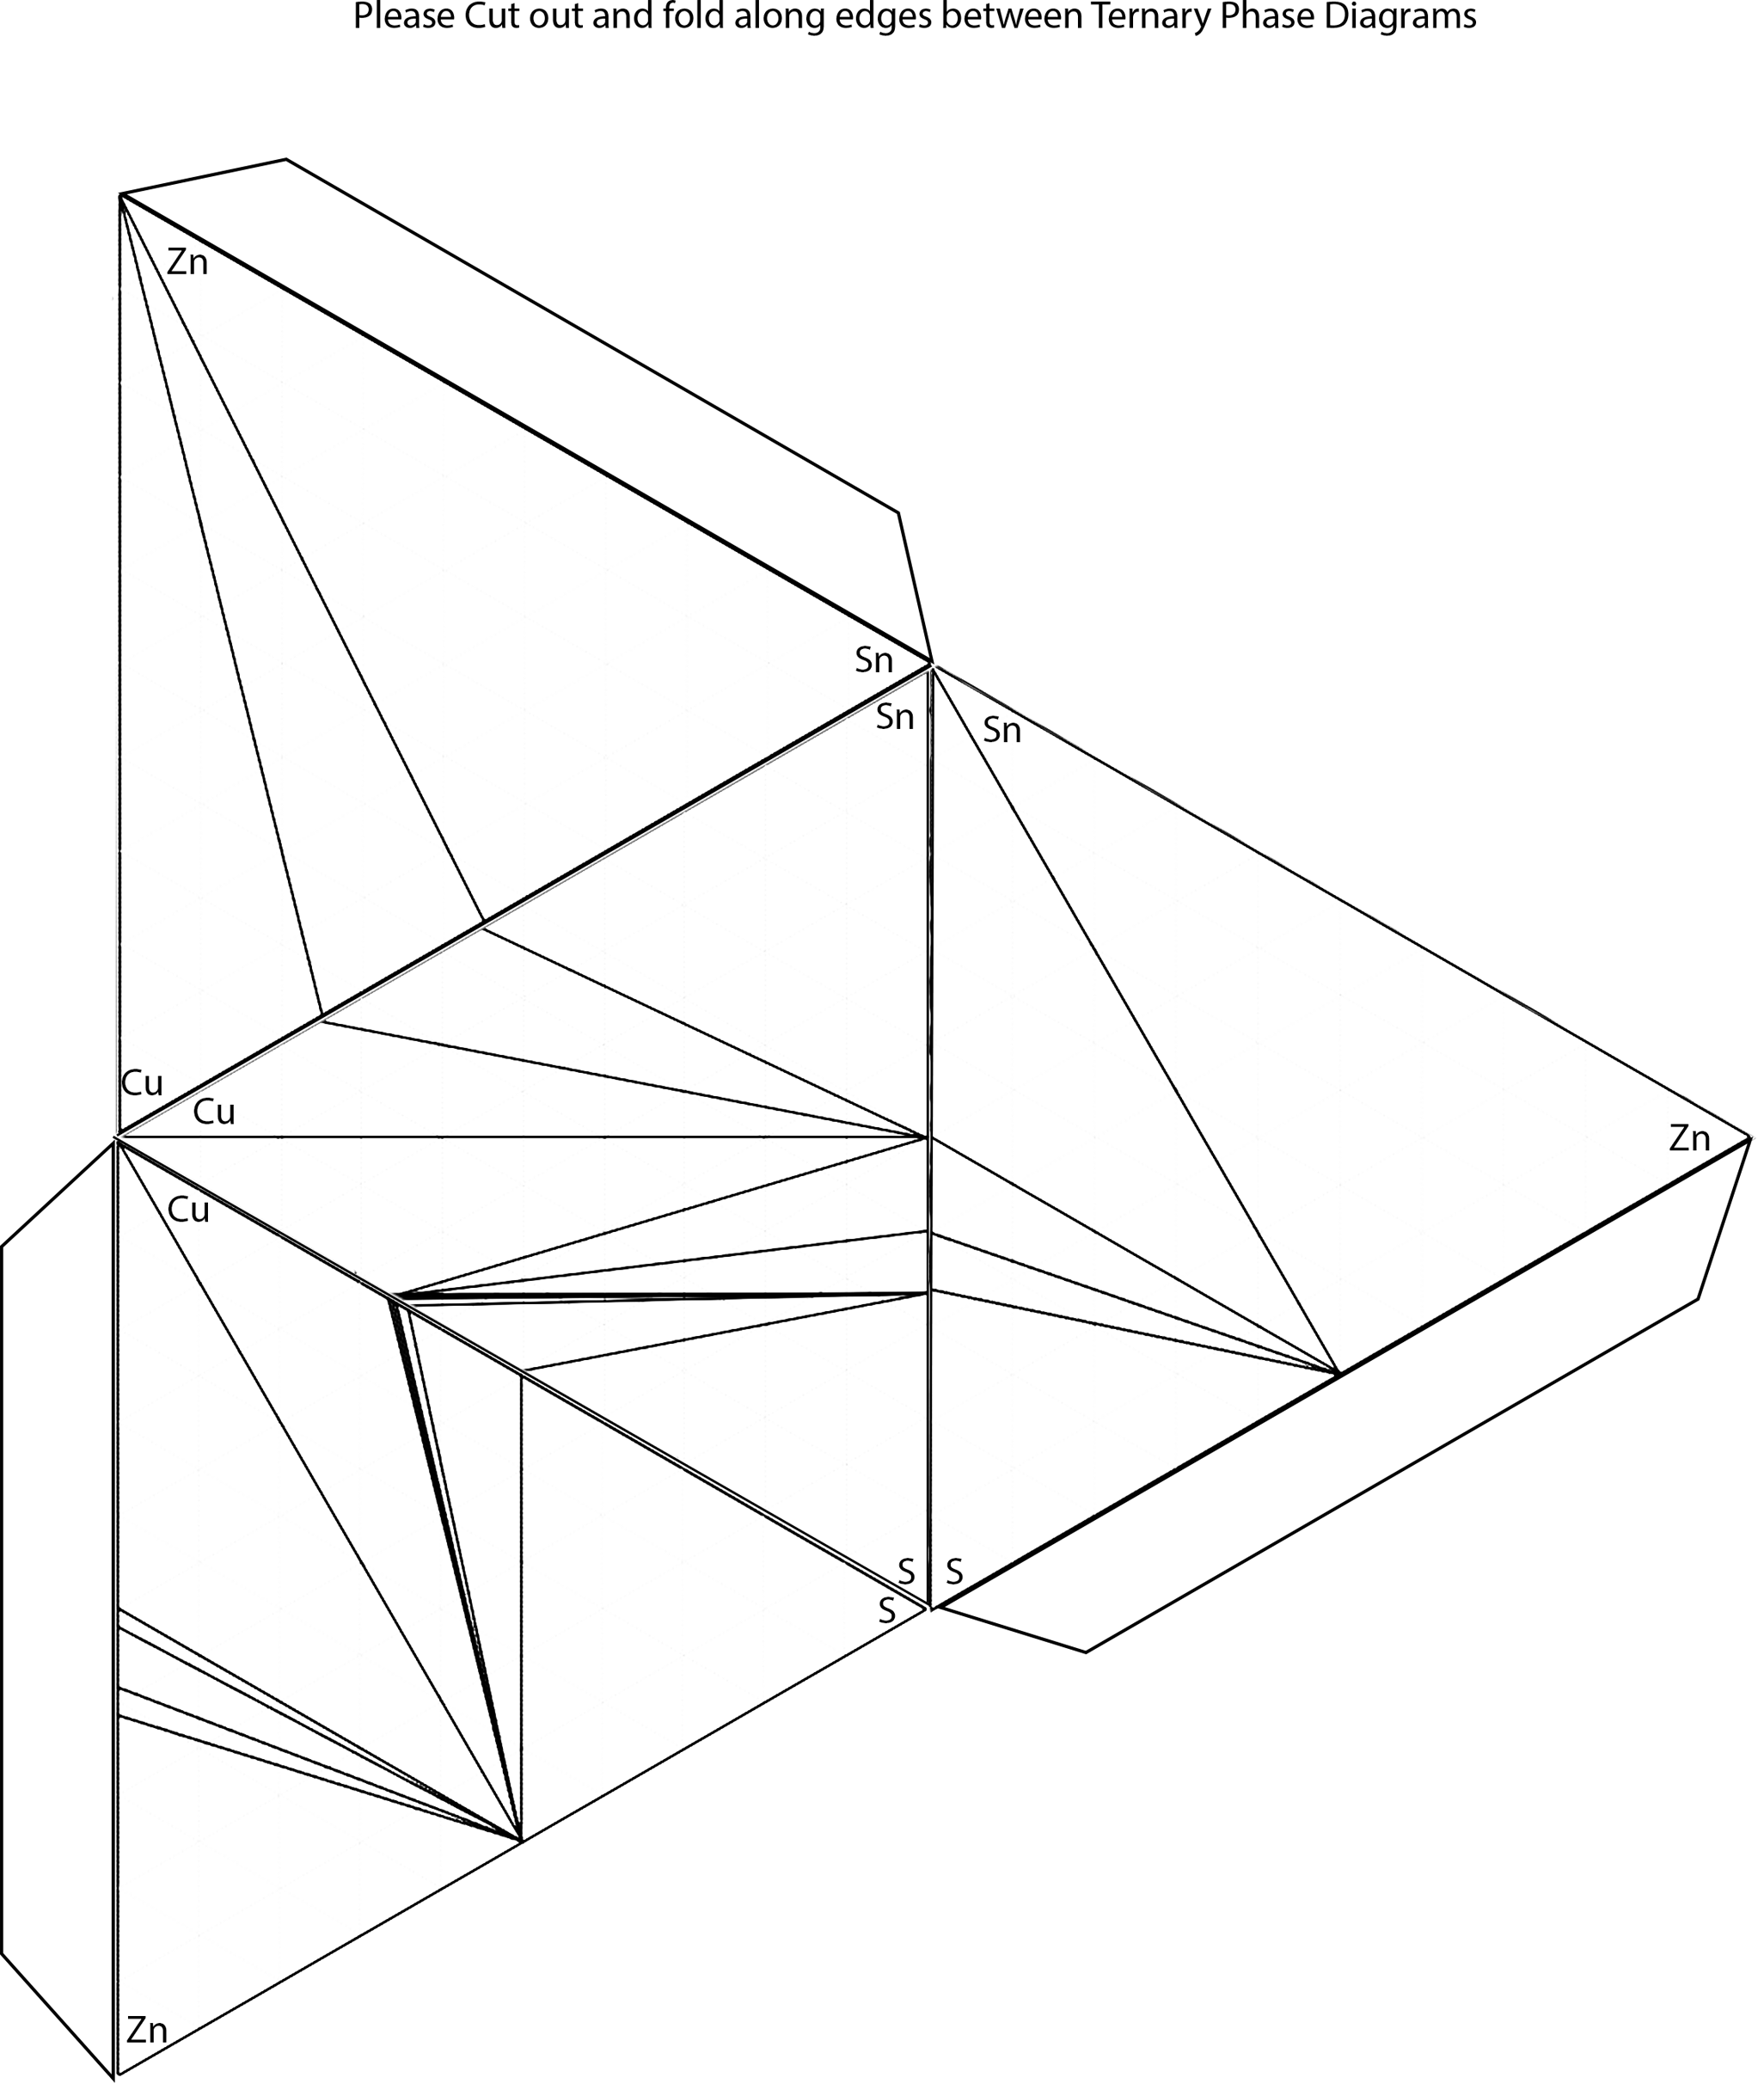
\includegraphics[width=160mm]{QPD-foldout}
\end{figure}

\addtocontents{toc}{\vspace{2em}} % Add a gap in the Contents, for aesthetics

\backmatter

\end{document}